\documentclass[11pt,a4paper,journal]{IEEEtran}

\usepackage{graphicx}
\usepackage{amsmath}
\usepackage{cite}

\title{Physics and Specifics for FPM \linebreak The Transmissive and Reflective Modes}
\author{Alankar~S.~Kotwal,~\IEEEmembership{Indian Institute of Technology Bombay}}

\begin{document}
\maketitle

\begin{abstract}
We model the optical system presented in \cite{FPMPaper} for Fourier Ptychographic Microscopy mathematically. The equations regarding the working of the system and phase retrieval are derived from first principles and an implementation in Matlab is discussed with its specifics. We then explore how the mathematics of the system changes when we move to imaging a reflective system, and specifically the human eye, using the same principles. An implementation for the reflective mode is then discussed.
\end{abstract}

\begin{keywords}
% Add more!
Fourier Ptychographic Microscopy, resolution improvement, Fourier optics, transmissive imaging, reflective imaging
\end{keywords}

\section{Introduction}
% Add more stuff
The throughput of a microscope is always limited by its optical system. It is not possible, conventionally, for a given optical system to perform beyond the limits set by Fourier optics (think diffraction). This means that the number of `uncorrelated' pixels one can extract out of the system is bounded. As we try to image features closer together, we come across correlations introduced by Fourier optics, which makes it impossible to resolve features more than a given spatial separation apart. Fourier Ptychographic Microscopy was introduced in 2013 as a computational tool to work around this.

The idea used in this method is to somehow shift the high-frequency information to low frequencies, where the system's optics will not filter it. Then we image the resulting object, and computationally form the final high-resolution image by `stitching together' the image in Fourier space using a phase retrieval algorithm. The advantage of this method is that we can perform this at low magnifications, still recover very high frequency information and hence acquire the ability to zoom in and see features to good resolution, resulting in a wide-field, high-resolution image.

This frequency shift is achieved using variable illumination. We illuminate the sample using LEDs at different locations below the sample (in the transmissive case). How this leads to a frequency shift is discussed in later sections. The lens filtering function is also characterised in later sections.

\section{Clearing Some Concepts}
These things must be kept in mind for what follows:
\begin{itemize}
\item \textit{What is the `image', and why is it complex?} The fields involved, are, of course not complex. We represent them as complex numbers to consider effects of phase (phasors). The image is the electric field transmittance at each pixel. Here, we realise the significance of the complex nature of the image. Fixing the phase at one pixel fixes the phases at all other pixels. We usually take phases to be zero at emission. This fixes phase at all points.
\item \textit{What do we measure?} We measure electric field intensity. This means, at every pixel, the energy received for the exposure time is recorded and stored. Hence, we are measuring $|\tilde{A}|^2$, where $\tilde{A}$ is the complex field at that pixel. This means, for obtaining the electric field magnitude from the measurements, we need to take a square root of the measurement images.
\item \textit{Why do we want the phase anyway?} Phase contains a lot of information about the physical nature of the diffracting aperture. So much so that swapping phase components of the Fourier transforms of two images keeping the amplitude images the same swaps visible features as well.
\end{itemize}

\section{The Transmissive System}

\subsection{The Physics}
We will now consider the FPM setup in the context of transmissive imaging. The standard setup here consists of a LED array illuminating a sample at a distance \textit{l}. This is followed by an imaging system, usually a microscope objective, that focusses light upon a detector. As the form of the final image will make clear, any image-forming system will do, as long as its magnification and bandwidth is known. We used a two-lens system to achieve this purpose. A Thorlabs DCx CCD camera (no optics) was the sensor used for imaging. The sample and the CCD have to be at conjugate planes for a focussed image. We assume that the distance from the sample to the objective lens is $f$, the focal length of the objective lens. The detector is placed at a distance $f'$, the focal length of the eyepiece, away from the eyepiece lens. All this is summarised in Fig. 1.

\begin{figure}
  \caption{The standard FPM setup}
  \centering
    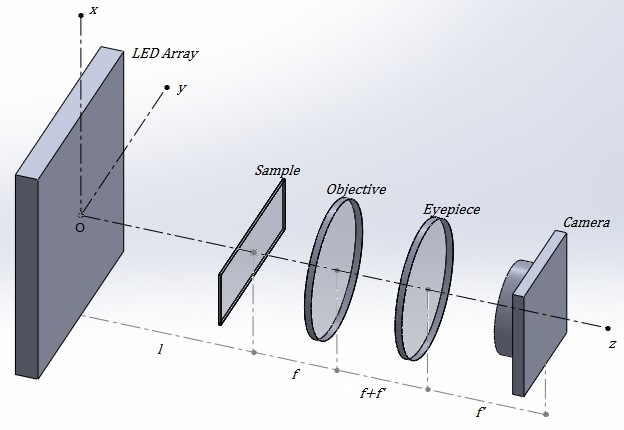
\includegraphics[scale=0.5]{FPM_Setup}
\end{figure}

Let us establish a coordinate system as shown in the figure. The origin lies on the optical axis at the LED array, which is centered on the optical axis. The $z$-axis coincides with the optical axis, the $x$-axis points vertically upward and the $y$-axis points into the plane of the paper.

Now consider an LED at coordinates $(x_l, y_l)$ on the $z=0$ plane illuminating the sample at the $z=l$ plane. The plane-wave phasor emitted by this LED will have the form
\begin{equation}
\tilde{E}(\vec{r}) = A e^{j \vec{k} \cdot \vec{r}}
\end{equation}
where the $\vec{k}$ represents the wavevector due to the LED at the sample and $j=\sqrt{-1}$. This is just a vector of magnitude $\frac{2\pi}{\lambda}$ pointing from the LED to the sample. Considering we're focussing on an area around coordinates $(x_s, y_s)$ in the sample $(z=l)$ plane, this is easily calculated, and the vector turns out to be
\begin{equation}
\vec{k} = \frac{2\pi}{\lambda} \frac{(x_s-x_l)\hat{x}+(y_s-y_l)\hat{y}+l\hat{z}}{\sqrt{(x_s-x_l)^2+(y_s-y_l)^2+l^2}}
\end{equation}

Once we have this, we can calculate the field configuration in the sample plane:
\begin{equation}
\begin{split}
\tilde{E}(x, y, l^-) & = A e^{j(k_x x + k_y y + k_z l)} \\
				   & = Ae^{jk_z l} e^{j(k_x x + k_y y)} \\
				   & = \tilde{A} e^{j(k_x x + k_y y)}
\end{split}
\end{equation}
The last equality follows from the fact that once $k_x$ and $k_y$ are known, $k_z$ is determined.

This electric field then passes through the sample. Assuming the sample is thin enough, the field is modulated by the transmittance function of the sample, which we want to estimate. Let the transmittance be $\Psi (x, y)$.
\begin{equation}
\tilde{E}(x, y, l^+) = \tilde{A} \Psi (x, y) e^{j(k_x x + k_y y)}
\end{equation}
%We will drop the $\tilde{A}$ from now on for convenience, since it is constant given $z$.

We now invoke the Fourier transforming property of lenses \cite[p.~104]{Goodman}, since the electric field configuration at the front focal plane of the lens is known. We neglect the lens pupil function for now. The field at the back focal plane is, thus, 
\begin{equation}
\begin{split}
\tilde{E}(x, y, d') &= \mathcal{F}[\tilde{A} \Psi (x, y) e^{j(k_x x + k_y y)}] \bigg|_{f_X=\frac{x}{f\lambda}, f_Y=\frac{y}{f\lambda}} \\
					  &= \tilde{A} \tilde{\Psi}\left(f_X - \frac{k_x}{2\pi}, f_Y - \frac{k_y}{2\pi}\right) \bigg|_{f_X=\frac{x}{f\lambda}, f_Y=\frac{y}{f\lambda}}
\end{split}
\end{equation}
where $\tilde{\Psi}(f_X, f_Y)$ is the Fourier transform in terms of spatial frequency variables $f_X$ and $f_Y$, and $d'=l+2f$. Proceeding, 
\begin{equation}
\tilde{E}(x, y, l+2f) = \tilde{A} \tilde{\Psi}\left(\frac{x}{f\lambda} - \frac{k_x}{2\pi}, \frac{y}{f\lambda} - \frac{k_y}{2\pi}\right)
\end{equation}

The detector, being on the conjugate plane on the other side of the (eyepiece) lens, images the Fourier transform of this, that is, a scaled and inverted version of the original image. If the eyepiece lens has a focal length $f'$, we have, again using the Fourier transforming property of lenses,
\begin{equation}
\begin{split}
\tilde{E}(x, y, d) &= \mathcal{F}[\tilde{E}(x, y, l+2f)] \bigg|_{f_X=\frac{x}{f\lambda}, f_Y=\frac{y}{f\lambda}} \\
&= \tilde{A} e^{-j\frac{f}{f'}\left(k_x x + k_y y\right)} \Psi\left(-x\frac{f}{f'}, -y\frac{f}{f'}\right)
\end{split}
\end{equation}
with $d=l+2f+2f'$.

This is consistent with the fact that the image formed is inverted and magnified by a factor of $\frac{f}{f'}$.

The intensity is, thus,
\begin{equation}
|\tilde{E}(x, y, d)|^2 = \left|\tilde{A} \Psi\left(-x\frac{f}{f'}, -y\frac{f}{f'}\right)\right|^2
\end{equation}

Equation (6) is how oblique illumination leads to a frequency shift. The information at spatial frequency $f_X = \frac{k_x}{2\pi}, f_Y = \frac{k_y}{2\pi}$ is brought to zero frequency.

Now we need to model the effect of the pupil function of the lens. The pupil function restricts the amount of light proceeding towards the camera to a circle of radius $r_{l}$. Thus, the following circular function gets multiplied pointwise with the electric field after passing through the lens:
\begin{equation}
circ(x, y) = \left\{
  \begin{array}{lr}
    1 & : \sqrt{x^2 + y^2} \le r_{l} \\
    0 & : \sqrt{x^2 + y^2} > r_{l}
  \end{array}
\right.
\end{equation}
This corresponds to a convolution in Fourier space with the corresponding Fourier transform. The Fourier transform of this circular function is
\begin{equation}
\mathcal{F}[circ(x, y)] = \frac{r_{l} J_1(2\pi r_l \sqrt{f_X ^2 + f_Y ^2})}{\sqrt{f_X ^2 + f_Y ^2}}
\end{equation}
where $J_1(x)$ is the Bessel function of the first kind with $\alpha=1$.

Now since we limit the source to a radius of $r_l$, we limit the frequency domain space to $\frac{r_l}{f\lambda}$. This is because the frequency domain and spatial domain are related by
\begin{equation*}
f_X=\frac{x}{f\lambda}, f_Y=\frac{y}{f\lambda}
\end{equation*}
This means, the radius of the circle around the center (the 'pupil') where the Fourier spectrum contains valid information is
\begin{equation}
r_p = \frac{r_l}{f\lambda}
\end{equation}
in units of spatial frequency.

Note that though we derived this for a two-lens system, the general form of the image will be
\begin{equation*}
\tilde{E}(x, y, d) = \tilde{A} e^{jm\left(k_x x + k_y y\right)} \Psi\left(xm, ym\right)
\end{equation*}
where $m$ is the signed magnification of the image-forming system, with $m$ negative in case of an inverted image. The pupil radius will be the bandwidth of the optical system.

The Fourier transform of the image in terms of the frequency coordinates $(f_X, f_Y)$ is given as 
\begin{equation}
\mathcal{F}[\mathcal{I}] = \tilde{A} \frac{f'^2}{f^2} \tilde{\Psi}\left(-\frac{k_x}{2\pi}-\frac{f_X f'}{f}, -\frac{k_y}{2\pi}-\frac{f_Y f'}{f}\right)
\end{equation}

It is clear from equation (12) that the frequency content from $(f_X, f_Y) = \left(\frac{-fk_x}{2\pi f'}, \frac{-fk_y}{2\pi f'}\right)$ in the normally illuminated image is brought to zero frequency when illuminated with the LED corresponding to $(k_x, k_y, k_z)$. This scale will also cause the pupil radius to fall by a factor of $\frac{f}{f'}$.

To accommodate the increased spatial resolution, we upsample all intensity images by a factor $m$ and take a square root to get field magnitudes. $m$ is chosen in a way that does not slow the calculation down (low values preferred) and so that we still have enough resolution to display features close by (high values preferred). A majority of times a value of $5$ to $10$ is observed to give good results. Note that after a bound\footnote{Calculate this bound!}, increasing $m$ will have no effect on image quality.

Phase retrieval is now easy. We initialize a guess image with the same size as the upsampled images. Now, according to the above analysis, the frequency content around $(f_X, f_Y) = \left(\frac{-fk_x}{2\pi f'}, \frac{-fk_y}{2\pi f'}\right)$ within a radius of $\frac{r_l}{f'\lambda}$ is shifted to zero frequency in a situation where the sample is illuminated at $(k_x, k_y, k_z)$. So we generate a new image in which this patch is at the center (zero frequency). According to our model, the magnitude (in the spatial domain) of this new image must be the measured magnitude corresponding to $(k_x, k_y, k_z)$. So we replace the magnitude of the (spatial domain) image by the measured magnitude. Then we transfer the patch in the (new) Fourier domain image back to its place in the guess image. We run this on all images and if required, more than once through the entire dataset, until convergence.

\subsection{The Implementation}
We know all characteristics of the image in the detector plane. We will perform all the phase retrieval in the detector plane itself.

Given the size per pixel, we need the per-pixel units for the Fourier transform. Since the input image is discrete, we need to use the discrete Fourier transform (DFT) to calculate the frequency domain image.  Now if the original image is sampled at a distance $\Delta x$ in one dimension, the DFT samples are taken at a separation of $\frac{1}{N\Delta x}$\cite{DFTWiki}, where $N$ is the size of the image (in pixels) in that dimension. Thus, a pixel at DFT coordinates $(u, v)$ from the center corresponds to a spatial frequency of $\left(\frac{u}{s_x}, \frac{v}{s_y}\right)$, where the size of the sensor is $s_x \times s_y$.

In practice, we also had to register the images to align features in the images. We cropped the edges of images so that no image had any part where there was no information. In that case, the denominator in the above expression will change to the effective detector dimension that was used in the cropped images.

\section{The Reflective System}
The same physics can be applied now to find how a light wave hitting an optically thick surface will diffract and get imaged on a camera.

\subsection{The Physics}
\begin{figure}
  \caption{The setup for the reflective case}
  \centering
    
\includegraphics[scale=1]{fpm_setup_refl}
\end{figure}
Fig. 2 shows the proposed setup for imaging reflective surfaces with this method.

\subsection{The Implementation}

\section{Future Work}

\begin{thebibliography}{10}

\bibitem{FPMPaper}
  Zheng, G et al.,
  \emph{Wide-Field, High-Resolution Fourier Ptychographic Microscopy}.
  Nature Photonics,
  2013.
  
\bibitem{FPMAnalysis}
  Horstmeyer, R. and Yang, C.,
  \emph{A Phase Space Model of Fourier Ptychographic Microscopy}.
  Optics Express,
  2014.
  
\bibitem{Goodman}
  Goodman, J.,
  \emph{Introduction to Fourier Optics}, Second Edition.
  McGraw-Hill Series in Electrical and Computer Engineering,
  1996.

\bibitem{DFTWiki}
  Wikipedia contributors,
  \emph{Discrete Fourier transform}.
  Wikipedia, The Free Encyclopedia,
  9 Dec. 2014
  
\end{thebibliography}


\end{document}